\documentclass[12pt]{article}

\usepackage[utf8]{inputenc}
\usepackage[spanish]{babel}
\usepackage[colorlinks=true ,linkcolor=red, urlcolor= red, citecolor= green]{hyperref}
\usepackage{graphicx}
\usepackage{amsmath}
\usepackage[a4paper, margin=1in]{geometry}
\spanishdecimal{.}
\usepackage{amssymb}


%tikzpicture
\usepackage{tikz}
\usepackage{scalerel}
\usepackage{pict2e}
\usepackage{tkz-euclide}
\usetikzlibrary{calc}
\usetikzlibrary{patterns,arrows.meta}
\usetikzlibrary{shadows}
\usetikzlibrary{external}

%pgfplots
\usepackage{pgfplots}
\pgfplotsset{compat=newest}
\usepgfplotslibrary{statistics}
\usepgfplotslibrary{fillbetween}


\author{Gups}
\date{\today}
\title{Oscilaciones y ondas}
\begin{document}
\maketitle

\begin{figure}[h]
    \centering
    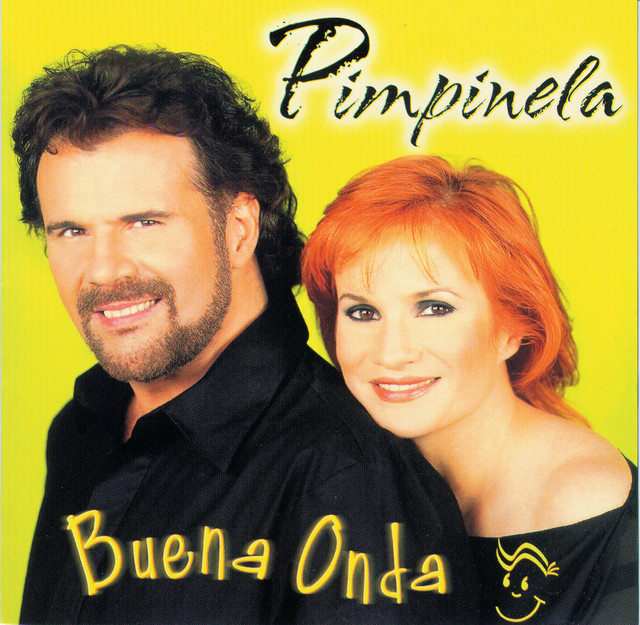
\includegraphics[width=10cm]{img/buena onda .jpeg}
\end{figure}

\newpage
\tableofcontents
\newpage


\section{Introducción}
Este apunte busca abordar lo temas tratados en el curso Oscilaciones y Ondas dictado por el profesor Renato Saavedra

\section{Características de una onda }

Una onda es un fenómeno físico el cual se describe la propagación de una perturbación a través del espacio, pueden o no requerir de un medio para transmitirse.

Alguna características importantes de las ondas son:\\

Se presentan como eventos periódicos(se repite un ciclo cada cierto tiempo)

\begin{figure}[h]
    \centering
    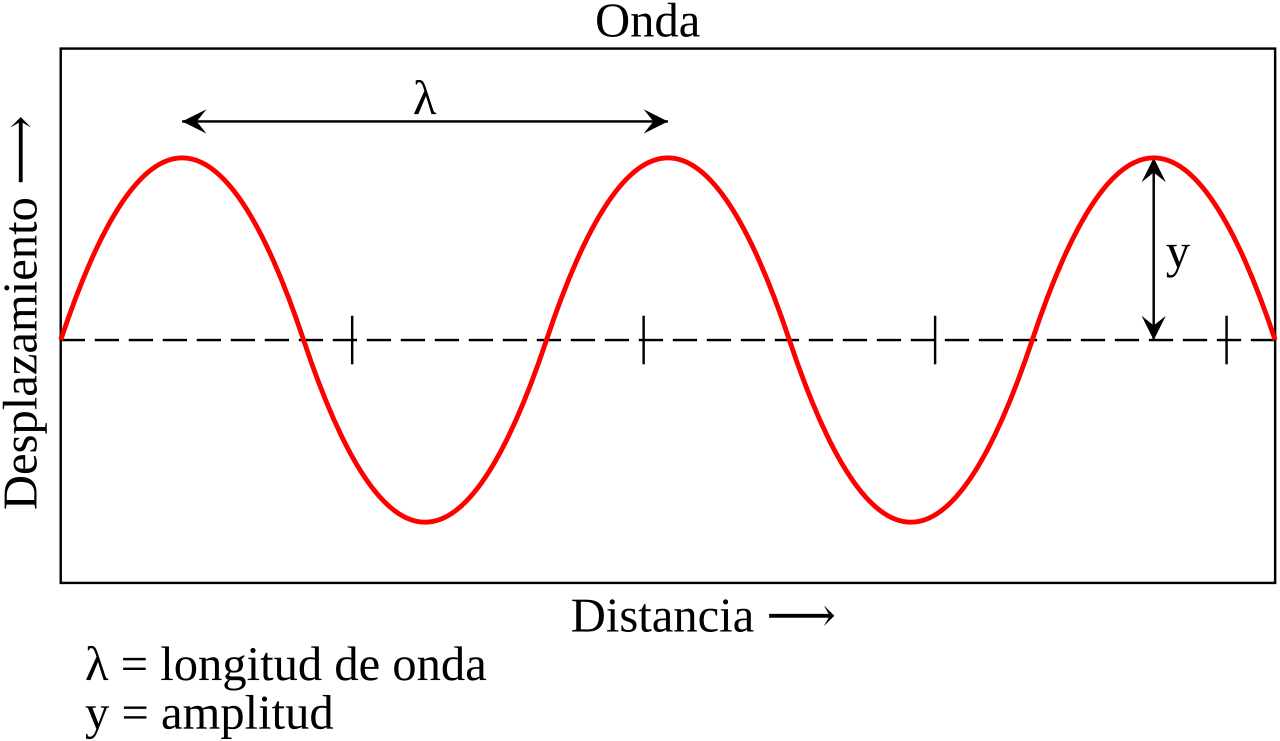
\includegraphics[width=0.8\textwidth]{img/Wave_characteristics.svg.png}
\end{figure}
\begin{itemize}
    \item \textbf{Amplitud }\((y)\):  Es la distancia vertical entre una cresta o valle y el punto de equilibrio de la onda. Nótese que pueden existir ondas cuya amplitud sea variable, es decir, crezca o decrezca con el paso del tiempo.
    \item \textbf{Longitud de onda }\((\lambda)\): Es la distancia que hay entre el mismo punto de dos ondulaciones consecutivas, o la distancia entre dos crestas, valles o tres nodos consecutivos.
    \item \textbf{Periodo }\((T)\): Es el tiempo empleado en completar una longitud de onda(oscilación completa).
    \item \textbf{Frecuencia }\((f)\): Es el número de periodos por unidad de tiempo. Es decir: el número de veces que es repetida dicha vibración por unidad de tiempo.
    \item \textbf{Velocidad de propagación }\((v)\): Es la velocidad a la que se propaga el movimiento ondulatorio. Su valor es el cociente de la longitud de onda y su período. 
\end{itemize}
\begin{align}
    T &= \frac{1}{f}   \label{eq: relacion-frecuencia-periodo}\\
    \lambda f &= v \label{eq: relacion-rapidez-frecuencia-lambda}
\end{align}

Como una onda representa un acontecimiento cíclico a veces es conveniente expresarla en términos de una frecuencia angular
\begin{align}
    \omega = 2\pi f
\end{align} 

\section{Oscilaciones}

Una oscilación corresponde a una variación periódica y armónica de alguna magnitud.\\

A pesar de que las oscilaciones son fenómenos distintos a las ondas, comparten muchas características en común(frecuencia, periodo, amplitud),la principal diferencia es que no se propagan en el espacio.


\section{Ecuación de movimiento para un oscilador armónico simple}

Existen distintas situaciones que cumplen con ser un movimiento armónico simple, en general tienen en común el describir movimientos periódicos producidos por alguna fuerza reconstitutiva que busca llevar el sistema a su posición de equilibrio, también en estos casos se considera que son sistemas en los que se conserva la energía, por lo tanto pueden oscilar infinitamente si nada se les opone.\\

En general pueden ser modelados bajo la siguiente ecuación de movimiento
\begin{align}
    m\ddot{x} + k \dot{x } = 0 ,\label{eq: movimiento-armónico-simple}\\
    \frac{dx}{dt} = \dot{x} \nonumber
\end{align}
esta ecuación se obtiene de aplicar segunda ley de Newton a un sistema cuya fuerza sea del tipo \( \sum F = ma = -kx\), donde \(x\) corresponde a la posición de la partícula donde se aplica la fuerza y \(k\) corresponde a la constante de elasticidad propia del sistema, puede  ser cualquier constante que relacione la posición con la fuerza.. El símbolo negativo en la expresión \(\sum F = - kx \) representa que la fuerza aplicada por el sistema va siempre en sentido contrario al sentido de su vector desplazamiento desde el punto de reposo \( x =  0\).\\

Las soluciones de esta ecuación diferencial, considerando \(k > 0 \) son del tipo 
\begin{align}
    x(t)&= A\cos\left(\sqrt{\frac{k}{m}}t\right) + B\sen\left(\sqrt{\frac{k}{m}}t\right),  \label{eq: solución-MAS}\\
     &= r \sen\left(\sqrt{\frac{k}{m}}t + \phi \right)  \label{eq: solución-MAS-variante seno}
\end{align}
la segunda ecuación viene de expresar \(A = r\sen(\phi) , B= r\cos(\phi)\) aplicar la identidad trigonométrica para la suma de ángulos. Asimismo, se comprueba que \(r= \sqrt{A^{2} + B^{2}} , \phi = \tan^{-1}(A/B)\). \\
Similarmente, haciendo el cambio de variable \(A= r \cos\phi\) y \(B = r\sen\phi\) se puede llegar a forma de solución
\begin{align}
    x(t) = r\cos\left( \sqrt{\frac{k}{m}}t + \phi \right) \label{eq: solución-MAS-variante seno}
\end{align}


De manera más general para cualquier sistema que presente una frecuencia de oscilación angular \(\omega\) su movimiento estará dado por, 
\begin{align}
    x(t) = r\sen(\omega t  + \phi),  \hspace{1cm} \phi = \tan^{-1}(x_{0}/v_{o})  \wedge r= \sqrt{v_{0}^{2} + x_{0}^{2}} \label{eq : x mas}
\end{align}

De todas maneras, la expresiones son equivalentes y se recomienda elegir cualquiera que sea más cómoda de trabajar en cada problema correspondiente. La principal ventaja de observar la solución en términos de \(r,\phi\) es notar que el movimiento mantiene su forma sinusoidal sin importar las condiciones de borde(condiciones iniciales). 


\newpage
\subsection*{Ejemplo: Sistema masa resorte vertical}
Suponga un resorte que cuelga del techo, en el extremo libre del resorte se cuelga una caja de masa \(m\) y se libera del reposo a una distancia \(y_0\) debajo su posición de equilibrio



\begin{figure}[h!]
    \centering
    \begin{tikzpicture}[black!75,thick]
 
% Supporting structure
\fill [pattern = north west lines](-3,0) rectangle ++(6,.2);
\draw[thick](-3,0) -- ++(6,0);
 
% Spring 1
\draw
[
    decoration={
        coil,
        aspect=0.3, 
        segment length=0.8mm, 
        amplitude=2mm, 
        pre length=3mm,
        post length=3mm},
    decorate
](-1.5,0) -- ++(0,-2) 
    node[midway,right=0.25cm,black]{$k$}; 
 % Spring 2
\draw
[
    decoration={
        coil,
        aspect=0.3, 
        segment length=1.2mm, 
        amplitude=2mm, 
        pre length=3mm,
        post length=3mm},
    decorate
](1.5,0) -- ++(0,-3) 
    node[midway,right=0.25cm,black]{$k$}; 
 
% Mass
\node[draw,
    fill=gray!60,
    minimum width=1cm,
    minimum height=0.75cm,
    anchor=north,
    label=center:$m$] at(1.5,-3) {};

%referencia

\draw[-Stealth,color=black](-5,-1) -- ++(0,1) node[right=0.2cm] {\(y\)};
\draw[-Stealth,color=black](-5,-1) -- ++(1,0) node[right=0.2cm] {\(x\)};

\draw[dashed](-3,-2) -- ++(6,0) node[right] {\(y=0\)};
 
\draw[dashed](-3,-3) -- ++(6,0) node[right] {\(y=-y_0\)};
%vectores
\draw[-Stealth,color=red](1.5,-3) -- ++(0,1) node[midway,right=0.3cm] {\(ky_0\)};
\draw[-Stealth,color=red](1.5,-3.75) -- ++(0,-0.8) node[midway,right=0.3cm] {\(mg\)};

\end{tikzpicture}
\end{figure}

Planteando segunda ley de Newton sobre la masa obtenemos
\begin{align*}
    m\ddot{y} = -ky - mg
\end{align*}
notar que la fuerza producida por el resorte no es constante, depende de la posición, luego resolviendo la EDO se llega a la solución general
\begin{align*}
    y(t) = A\sen(\omega t ) + B \cos( \omega t) - \frac{mg}{k} , \qquad \omega = \sqrt{k / m} 
\end{align*}
Luego, imponiendo condiciones iniciales obtenemos que \(A=0, B = y_0 + \frac{mg}{k}\), por lo que la ecuación de movimiento del sistema masa resorte vertical queda
\begin{align*}
    y(t) = \left(-y_0 + \frac{mg}{k}\right)\cos(\omega t) - \frac{mg}{k}
\end{align*}
\section{Velocidad y aceleración de un MAS(movimiento armónico simple)}
Derivando respecto al tiempo obtenemos ecuaciones para la velocidad y aceleración de un oscilador armónico
\begin{align}
    \dot{x} = \omega r \cos(\omega t + \phi), \label{eq : velocidad-mas} \\
    \ddot{x} = -\omega^{2} r \sen(\omega t + \phi) \label{eq: aceleracion-mas}
\end{align}

Considerando la ecuación \eqref{eq: aceleracion-mas} podemos recuperar la segunda ley de Newton planteada originalmente en el ejemplo anterior.

\section{Energía en un oscilador}

Recordemos que la energía de un sistema mecánico puede expresarse como la suma de la energía cinética \(K\) más una energía potencial \(U\), de forma que en todo instante la energía total \(E\) está dada por 
\begin{align}
    E &= K + U \nonumber\\
    E &= \frac{1}{2}m v^{2} + U
\end{align}
Generalmente, la energía potencial puede escribirse como
\begin{align*}
    U(x,y,z) &= - \int_{\vec{a}}^{\vec{x}} \vec{F} \cdot d\vec{\ell} \\
    &= -\left(\int_{\vec{a}}^{\vec{x}} F_x(x,y,z) dx + \int_{\vec{a}}^{\vec{x}} F_y(x,y,z) dy + \int_{\vec{a}}^{\vec{x}} F_z(x,y,z) dz\right)
\end{align*}
Con \(\vec{F}\) las fuerzas conservativas del sistemas(ej: fuerza elástica, fuerza gravitacional, fuerza eléctrica)\\

Esta definición arrastra consigo una constante de integración \(U(\vec{a})\), la cual por convención adopta el valor 0 pues no tiene mayores implicancias físicas. En la practica, puede ser conveniente usar un valor distinto a 0 para simplificar cálculos algebraicos.\\


Como en un sistema que oscila la velocidad pasa de ser máxima para el desplazamiento \(x= 0\) y mínima para el desplazamiento máximo, podemos notar el intercambio que se realiza entre energía cinética y potencial en cada momento ,si además consideramos la conservación de la energía tenemos
\begin{align*}
    E_{\text{total}} = K + U = U_{\text{max}} = K_{ \text{max}} 
\end{align*}
esto también puede verse reflejado en que la amplitud de oscilación no disminuye a medida que avanzan los ciclos \( x = r\sen(\omega t + \phi)\).
\subsection{Energía potencial de un oscilador}
Corresponde a todo el trabajo posible a realizar por la fuerza interna del sistema con el objetivo de volver al estado de reposo,  así para un sistema de resorte con el origen de coordenadas en la posición natural de reposo del mismo, la energía potencial es
\begin{align*}
    U(x) = \int_{0}^{x} kx \cdot dx = \frac{1}{2 }kx^{2}
\end{align*}
Luego la energía potencial máxima esta dada por el máximo desplazamiento posible \(r\), 
\begin{align}
    U_{ \text{max}} = \frac{1}{2}kr^{2} \nonumber
\end{align}
\subsection{Energía cinética}
La energía cinética del sistema esta dada por
\begin{align*}
    E_c = \frac{1}{2}mv^{2}
\end{align*}
luego reemplazando el valor de magnitud máxima para la velocidad se obtiene, 
\begin{align*}
    v_\text{max} &= \dot{x}_\text{max} \\
    &= \text{max}(r\omega\sen(\omega t + \phi)) \\
    &= r\omega 
\end{align*}
\begin{align*}
    K_{\text{max}} = \frac{1}{2}m(\omega r )^{2} = \frac{1}{2}m \omega^{2} r^{2}
\end{align*}
\subsection{Ecuación de la energía total}
Para un sistema mas, para el que se conserva la energía se  cumple lo siguiente,
\begin{align}
    E = \frac{1}{2} m \dot{x}^{2} + \frac{1}{2}kx^{2}
\end{align}
reemplazando con la solución general del movimiento armónico \eqref{eq: solución-MAS-variante seno}
\begin{align*}
    E &= \frac{1}{2} m r^{2}\omega^{2} \cos^{2}(\omega t + \phi) + \frac{1}{2} k r^{2}\sen^{2}(\omega t + \phi), \quad \omega^{2} = \frac{k}{m} \\
    &= \frac{1}{2}k r^{2}
\end{align*}
También podemos igualar amabas energías máximas,
\begin{align*}
    \frac{1}{2}mr^{2}\omega^{2} = \frac{1}{2}kr^{2},\\
    \omega^{2} = \frac{k}{m}
\end{align*}
lo que nos devuelve la ecuación para la frecuencia angular de oscilación.
\section{Conservación de la energía y ecuación de movimiento}
Podemos comprobar que la energía del sistema se mantiene constante, esto es 
\begin{align*}
    \frac{d}{dt} E =0, \\
    m\dot{x}\ddot{x} + kx\dot{x} = 0, \\
(m\ddot{x} + kx)\dot{x} = 0, 
\end{align*}
Ahora, como la ecuación de movimiento del sistema es precisamente \(m\ddot{x} + k x = 0\), podemos concluir que se conserva la energía
\section{Oscilaciones en un circuito LC}
Para un sistema eléctrico que posee una inductancia \(L\) y una capacitancia \(C\) como el que se muestra en la figura \ref{fig: circuito lc} podemos plantear una EDO para la carga \(q\) en el circuito considerando que \(V_{L} = L \frac{d^{2}q}{dt^{2}} , \ V_C = \frac{q}{C}\) y utilizando la ley de Kirchhoff para el Voltaje, de modo que obtenemos

\begin{align*}
    L\ddot{q} + \frac{q}{C} = 0,
\end{align*}
o 
\begin{align*}
    \ddot{q} + \omega^{2}q = 0
\end{align*}
con \[\omega^{2} = \frac{1}{LC}\]
\begin{figure}
    \centering
    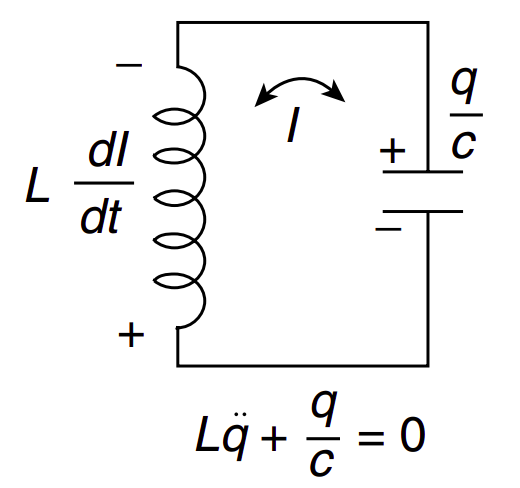
\includegraphics[width=4cm]{img/circuito LC.png}
    \caption{Circuito LC}
    \label{fig: circuito lc}
\end{figure}

\section{Puntos de equilibrio y aproximación para identificar sistemas oscilantes}

La razón por la que un sistema tiene a presentar oscilaciones que la existencia de una fuerza dirigida hacia un punto de equilibrio \(\sum \vec{F } = 0\)\\

Por simplicidad consideremos un potencial dependiente de una única coordenada \(U(x)\), le relación entre el potencial y la fuerza ejercida es
\begin{align*}
    -\frac{d U(x)}{d x} \hat{x} = F \hat{x}
\end{align*}
 Luego, un punto de equilibrio es aquel que cumple la condición
 \begin{align*}
    \frac{dU(x)}{dx} = 0
 \end{align*}

La condición para que un punto de equilibrio sea considerado estable es que la fuerza ejercida por el sistema alrededor del punto de equilibrio apunte en la dirección del punto de equilibrio

\begin{figure}[h]
    \centering
    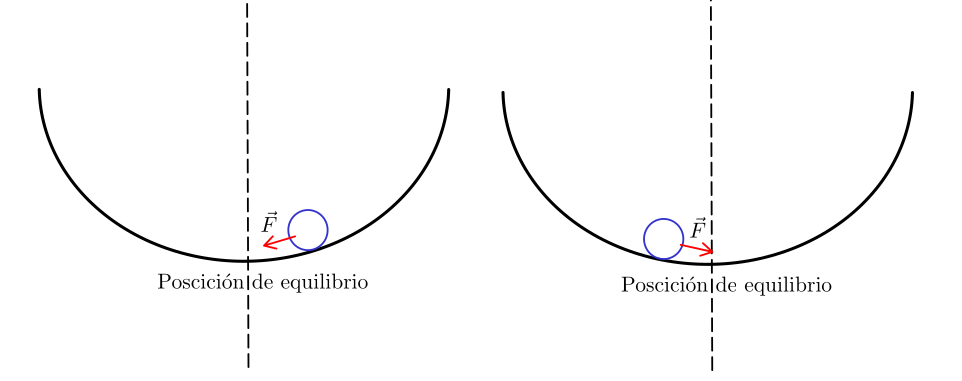
\includegraphics[width= 0.8\textwidth]{img/posición de equilibrio.png}

\end{figure}
Esta condición se cumple cuando el punto de equilibrio corresponde a un mínimo local en la energía potencial, la mayoría de las veces esta condición puede verificarse por medio de la segunda derivada de \(U\). Explícitamente, podemos decir
\begin{align*}
    \frac{d^{2}U(x)}{dx^{2}} \Bigg|_a > 0 \Rightarrow a \text{ es un punto de equilibrio estable}
\end{align*}


Con esta consideración podemos mostrar que cualquier sistema conservativo debiera oscilar al experimentar pequeñas perturbaciones alrededor de un punto de equilibrio estable.\\

Para ello expresaremos el potencial series de Taylor al rededor del punto \(x=a\), con \(a\) un punto de equilibrio estable
\begin{align*}
    U(x) = U(a + \Delta x), \qquad \Delta x :=(x-a)
\end{align*}
\begin{align*}
    U(x) = U(a) + \frac{dU}{dx} \Bigg|_a \Delta x + \frac{1}{2!}  \frac{d^{2}U(x)}{dx^{2}} \Bigg|_a(\Delta x)^{2} + \mathcal{O}(\Delta x ^{3})
\end{align*}
Como \(a\) es un punto de equilibrio, el segundo término es nulo, como además es estable, el tercer término es positivo.

reemplazando en la segunda ley de Newton
\begin{align*}
    m\ddot{x} &= - \frac{dU(x)}{dx}, \\
    m\ddot{x} &= -\frac{d^{2}U(x)}{dx^{2}} \Bigg|_a \Delta x + \mathcal{O}(\Delta x ^{3})
\end{align*}
Para perturbaciones pequeñas podemos ignorar los términos de orden superior y se recupera la ecuación de movimiento armónico simple en torno a el punto \(a\).\\

Puede ser útil expresar todo en términos de \(\Delta x\), para ello notamos la regla de la cadena
\begin{align*}
    \frac{d^{2} \Delta  x }{dt^{2}}=\frac{d}{dt}\left(\frac{d(x-a)}{dx} \frac{dx}{dt}\right) =  \frac{d^{2}  x }{dt^{2}}
\end{align*} 

Con lo que la ecuación de movimiento quedaría
\begin{align*}
    m\ddot{(\Delta x)} + \frac{d^{2}U(x)}{dx^{2}} \Bigg|_a \Delta x = 0\\
    m\ddot{(\Delta x)} + k_\text{eff}\Delta x = 0
\end{align*}
Donde \(\displaystyle \frac{d^{2}U(x)}{dx^{2}} \Bigg|_a\) recibe el nombre de constante efectiva.


\newpage

\section{Péndulo simple}
\begin{tikzpicture}
    \draw[-Stealth,color=black](-5,-1) -- ++(0,1) node[right=0.2cm] {\(y\)};
\draw[-Stealth,color=black](-5,-1) -- ++(1,0) node[right=0.2cm] {\(x\)};
\end{tikzpicture}
\begin{figure}[h!]
    \centering
    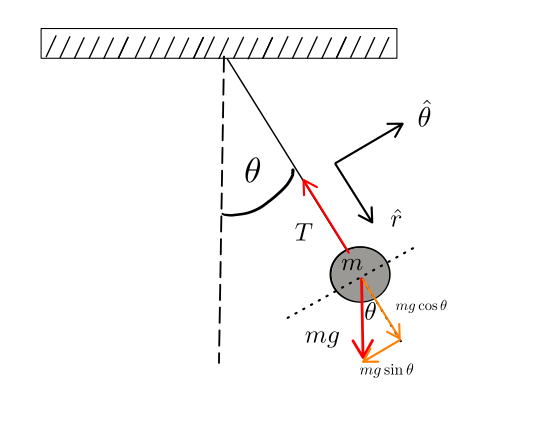
\includegraphics[width=5cm]{img/Pendulo xournal.png}
    \caption{Péndulo Simple} 
    \label{fig: Pendulo simple}
\end{figure}


El problema del péndulo es conveniente de tratar en coordenadas polares, para ellos definimos la transformación de coordenadas
\begin{align*}
    x&= r\sen\theta\\
    y&= -r\cos\theta, \qquad r \geq 0  \ \land \theta \in (-\pi,\pi]
\end{align*}
Definamos los vectores unitarios en nuestro sistema de coordenadas polares
\begin{align*}
    \hat{r} &= \sen\theta \hat{x} - \cos\theta \hat{y}\\
    \hat{\theta} &= -\cos\theta \hat{x} + \sen\theta \hat{y}
\end{align*}

Como el largo del péndulo es constante \(L\), entonces el vector posición y sus derivadas quedan 
\begin{align*}
    \vec{r}&= L\sen\theta \hat{x} - L\cos\theta \hat{y} = L\hat{r}\\
    \vec{v} &= L\dot{\theta}(\cos\theta \hat{x } + \sen\theta \hat{y}) = L\dot{\theta} \hat{\theta}\\
    \vec{a} &= L\ddot{\theta}(\cos\theta \hat{x } + \sen\theta \hat{y}) + L\dot{\theta}^{2}(-\sen\theta \hat{x} + \cos\theta\hat{y}) = L\ddot{\theta} \hat{\theta} - L\dot{\theta}^{2} \hat{r}
\end{align*}



Acá debemos analizar el diagrama de fuerzas de la figura \ref{fig: Pendulo simple} para notar que la fuerza resultante es la suma de la fuerza centrípeta con la fuerza tangencial
\begin{align*}
   \sum \vec{F} = -mg\sen\theta \hat{\theta} - m \frac{v^{2}}{L} \hat{r}
\end{align*}
Para una partícula en movimiento circular también se cumple la relación entre la rapidez y la rapidez angular
\begin{align*}
    v = L\omega = L \dot{\theta}
\end{align*}
Reemplazando esta forma tenemos
\begin{align*}
    \sum \vec{F} = -mg\sen\theta \hat{\theta} - m L\dot{\theta}^{2} \hat{r}
\end{align*}
aplicando segunda ley de Newton
\begin{align*}
     mL\ddot{\theta} \hat{\theta} - mL\dot{\theta}^{2} \hat{r} &= -mg\sen\theta \hat{\theta} - m L\dot{\theta}^{2} \hat{r}\\
     \rightarrow L\ddot{\theta} + g\sen\theta &= 0
\end{align*}
Para ángulos de oscilación pequeños se aproxima \(\sen\theta \approx \theta\) de modo que se obtiene la ecuación de movimiento armónico simple
\begin{align*}
    \ddot{\theta} + \frac{g}{L}\theta = 0
\end{align*}
Con solución
\begin{align*}
    \theta(t) = A \sen(\omega t + \phi) ,  \quad \omega = \sqrt{\frac{g}{L}}
\end{align*}
De esto se puede desprender que la frecuencia de oscilación de un péndulo depende de el largo de la cuerda y de la aceleración de gravedad, pero no de la masa

\subsubsection*{Otro acercamiento al problema}

Usualmente es más sencillo establecer que la posición de la masa queda determinada por la posición de segmento circular
\begin{align*}
    x = L \theta
\end{align*}
Como el radio es constante la aceleración queda
\begin{align*}
    a = \ddot{x} = L \ddot{\theta}
\end{align*}
De la segunda ley de Newton tenemos 
\begin{align*}
    mL\ddot{\theta} = -mg\sen\theta
\end{align*}
Con lo que se llega a la misma ecuación de movimiento para el ángulo \(\theta\)
\section{Péndulo físico y  Momento de inercia}

Para analizar el movimiento de un péndulo cuya distribución de masa varíe de la de un péndulo ideal, podemos analizar su movimiento en base a su centro de masa y el punto pivote(donde se encuentra el eje de giro) \\
\subsection{Centro de masa}


El centro de masa de un cuerpo puede obtenerse como un promedio ponderado de los vectores posición de las masas que contiene el sistema
\begin{align}
    \vec{R}_\text{cdm} = \frac{\sum_i m_i \vec{r_i}}{\sum_i m_i} = \frac{\sum_i m_i \vec{r_i}}{ M} \label{eq: centro de masa}
\end{align} 
Generalizando para sistemas continuos de masa 
\begin{align*}
    \vec{R} = \frac{\int dm \vec{r}}{M}, \quad dm = \rho dV
\end{align*}
Donde \(dm \) es un diferencial de masa y \(\rho \) es la densidad volumétrica de masa \\

El movimiento de un cuerpo físico puede representarse mediante traslaciones del centro de masa y sus rotaciones correspondientes.
\subsection{Momento de inercia} 
El momento de inercia de un cuerpo es una medida de que tan difícil es hacerlo rotar, para sistemas discretos se define como 
\begin{align}
    I = \sum_i m_i r_i^{2} \label{eq: momento de inercia}
\end{align}
Donde \(r_i\) es la distancia al eje de giro, por ejemplo en el caso del péndulo simple, como consiste de una sola partícula que gira en torno al punto pivote, su momento de inercia sería \(mL^{2}\)\\

Para sistemas continuos el momento de inercia se calcula como siguiente
\begin{align*}
    I = \int dm r^{2} = \int r^{2} \rho dV
\end{align*}
Es importante notar que para un mismo cuerpo, el momento de inercia puede cambiar si cambia la posición u orientación del eje de giro.

\begin{figure}[h]
    \centering
    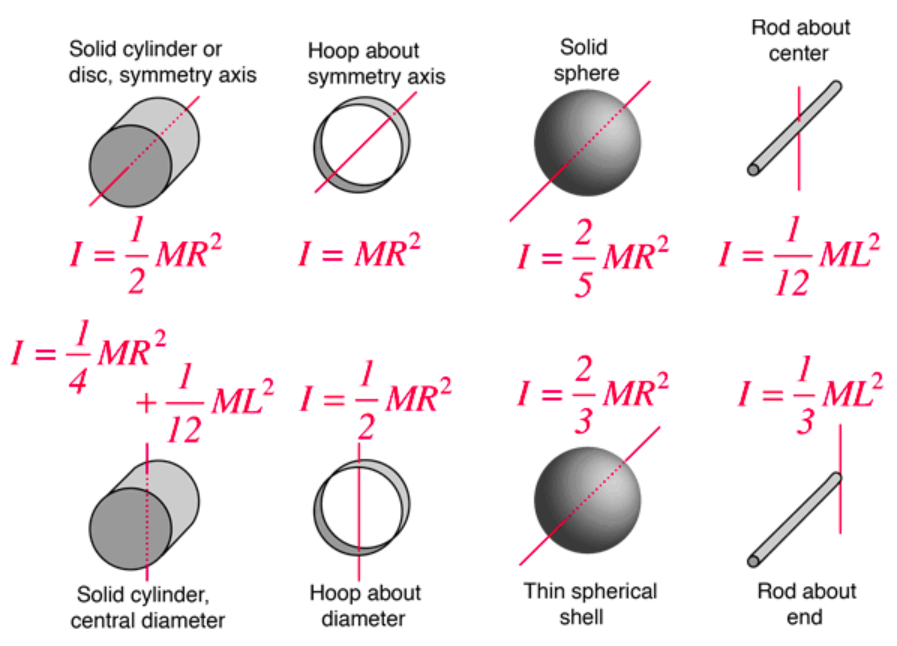
\includegraphics[width=0.7\textwidth]{img/Momentos de inercia.png}
    \caption{Ejemplos de algunos momentos de inercia }
\end{figure}
El momento de inercia también establece la relación entre el torque y la aceleración angular en rotaciones
\begin{align}
    \vec{\tau} = \vec{r} \times \vec{F} \label{eq: torque}
\end{align}
\begin{align}
    \sum \vec{\tau} = I \vec{\alpha}, \quad \alpha = \ddot{\theta} \label{eq : segunda ley de newton roaciones}
\end{align}
\subsection{Teorema de ejes paralelos(momento de inercia en un punto distinto al centro de masa)}
La relación entre el momento de inercia correspondiente a un eje de rotación posicionado en el centro de masa de un cuerpo \(I_{\text{cm}}\) y el momento de inercia correspondiente a cualquier otro eje de rotación que sea paralelo al eje del centro de masa y esta a una distancia \(d\) está dada por:
\begin{align}
    I = I_{\text{cm}} + md^{2}
\end{align} 

\subsection{Péndulo físico}

\begin{figure}[h!]
    \centering
    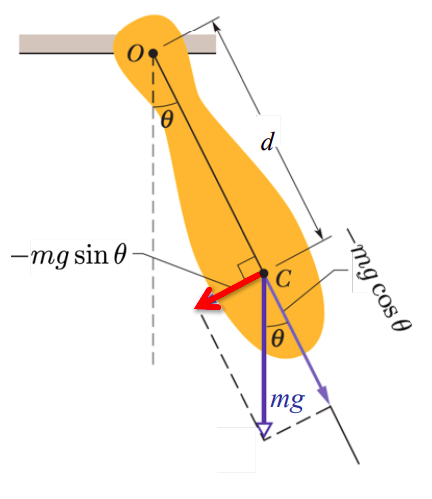
\includegraphics[width=5cm]{img/Pendulo fisico.png}
    \caption{Péndulo físico}
    \label{fig; pendulo-fisico}
\end{figure}
Aplicando la segunda ley de Newton para rotaciones \eqref{eq : segunda ley de newton roaciones} tenemos
\begin{align*}
    I\ddot{\theta} = -mgd\sen\theta\\
    \rightarrow \ddot{\theta} + \frac{mgd}{I}\sen\theta = 0
\end{align*}
Nuevamente, para ángulos pequeños se obtiene la ecuación del oscilador armónico simple
\begin{align*}
    &\ddot{\theta} + \frac{mgd}{I}\theta = 0, \\
    \rightarrow &\theta(t) = A \sen(\omega t + \phi) , \quad \omega = \sqrt{\frac{mgd}{I}}
\end{align*}
Con esto se puede despejar el periodo de un péndulo físico como 
\begin{align*}
    T = 2\pi\sqrt{\frac{I_p}{mgd}}
\end{align*}
Donde \(I_p\) corresponde al momento de incercia en el pivote, \(m\) es la masa del péndulo, \(d \) es la distancia del centro de masa al punto pivote y \(g\) la aceleración de gravedad
\section{Superposición de oscilaciones}
Existen distintas formas en las que movimientos armónicos pueden superponerse(interferencia), la clasificación y análisis de estas dependerá de la frecuencia y dirección de las oscilaciones

\subsection{Superposición de oscilaciones en la misma dirección/colineales } \label{subsec: superpocición de oscilaciones colineales}

Sean dos movimientos armónicos en la misma dirección \(x_1(t), x_2(t)\)
\begin{align*}
    x_1(t) = A_1\sen(\omega_1 t + \phi_1) \\
    x_2(t) = A_2\sen(\omega_2 t + \phi_2)
\end{align*}

El movimiento resultante responde al principio de superposición, es decir, corresponderá a la suma directa de las  funciones, para obtener un resultado útil es necesario conocer la siguiente identidad trigonométrica.\\

Partiendo de que para cualquier par de números reales \(A\) y \(B\) es posible realizar la sustitución \(A= \alpha + \beta,  B= \alpha - \beta\)
\begin{align*}
    &C_1\sen A + C_2\sen B \\
     =& C_1\sen(\alpha +\beta) + C_2\sen(\alpha-\beta)\\
    =&(C_1 + C_2)\sen\alpha\cos\beta +(C_1 - C_2)\sen\beta\cos\alpha
\end{align*}
Con
\begin{align*}
    \alpha = \frac{A+ B }{2} \text{y} \ \beta = \frac{A-B }{2}
\end{align*}
De esta forma
\begin{align*}
    &x_1(t) + x_2(t) =\\
    &=(A_1 + A_2)\sen\left(\frac{(\omega_1 + \omega_2)t + \phi_1 + \phi_2}{2}\right)\cos\left(\frac{(\omega_1 - \omega_2)t + \phi_1 - \phi_2}{2}\right)\\
     & \quad +(A_1 - A_2)\sen\left(\frac{(\omega_1 - \omega_2)t + \phi_1 - \phi_2}{2}\right)\cos\left(\frac{(\omega_1 + \omega_2)t + \phi_1 + \phi_2}{2}\right)
\end{align*}
Si bien esta es la expresión más general, hay casos más sencillos que es interesante resaltar
\subsubsection*{Caso \(\omega_1 = \omega_2 = \omega\) }
\begin{align*}
    &x_1(t) + x_2(t) =\\
    &=(A_1 + A_2)\sen\left( \omega t +\frac{ \phi_1 + \phi_2}{2}\right)\cos\left(\frac{ \phi_1 - \phi_2}{2}\right)\\
     & \quad +(A_1 - A_2)\sen\left(\frac{ \phi_1 - \phi_2}{2}\right)\cos\left(\omega t +\frac{ \phi_1 + \phi_2}{2}\right)
\end{align*}

Como \(\phi_1,\phi_2\) son constantes esta solución resulta en
\begin{align*}
    x_1(t) + x_2(t) = \tilde{A}_1\sen\left( \omega t +\frac{ \phi_1 + \phi_2}{2}\right) + \tilde{A}_2\cos\left(\omega t +\frac{ \phi_1 + \phi_2}{2}\right)
\end{align*}
Lo que es simplemente otro movimiento oscilatorio de la misma frecuencia.\\

Dentro de este caso es interesante notar que si \(A_1 = A_2\) y \(\phi_1 - \phi_2 =(2k+1)\pi\) entonces se obtiene una interferencia perfectamente destructiva.

\subsubsection*{Caso \(A_1 = A_2 = A\)}

\begin{align*}
    &x_1(t) + x_2(t) =\\
    &= 2A \sen\left(\frac{(\omega_1 + \omega_2)t + \phi_1 + \phi_2}{2}\right)\cos\left(\frac{(\omega_1 - \omega_2)t + \phi_1 - \phi_2}{2}\right)\\
\end{align*}
Esta caso resulta en el producto de un seno de mayor frecuencia por un coseno de menor frecuencia que acota superior e inferiormente los valores de la onda resultante, Este fenómeno se conoce como \textbf{beating} y suele ser más notorio cuando los valores de frecuencias son similares entre si \(\omega_1 \approx \omega_2\).\\

Pueden probar variar los parámetros en geogebra para ver como se manifiesta este efecto \url{https://www.geogebra.org/classic/z4pwjft5}

\subsection{Superposición de oscilaciones perpendiculares}
\begin{align*}
    x(t) = A_x\sen(\omega_x t + \phi_x) \\
    y(t) = A_y\sen(\omega_y t + \phi_y)
\end{align*}


Este tipo de superposición resulta en la formación de figuras en el plano la cuales pueden ser parametrizadas como figuras de Lissanjou

\begin{figure}[h!]
    \centering
    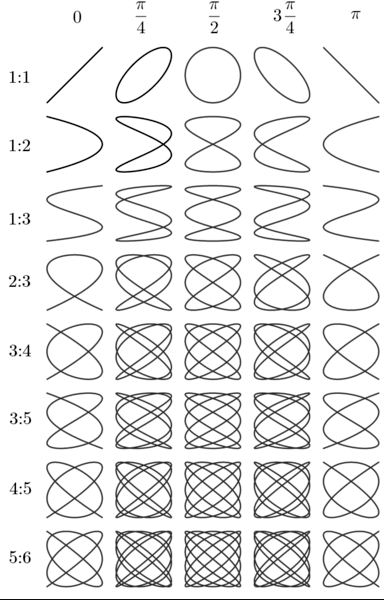
\includegraphics[width = 7cm]{img/Lissanjou.png}
    \caption{Figuras de Lissanjou}
\end{figure}


\newpage
\section{Oscilaciones amortiguadas}
Corresponden a aquellas que surgen de algún sistema físico en el cual la velocidad de un cuerpo o partícula provoca una fuerza de resistencia en contra del movimiento y cuya magnitud es proporcional a rapidez(en el caso de un roce viscoso, puede variar, por ejemplo para la resistencia del aire la fuerza es proporcional a \(v^{2}\)).\\

Aplicando la segunda ley de Newton para un cuerpo que oscila con la acción de un roce viscoso obtenemos la siguiente ecuación
\begin{align}
    \sum \vec{F} = m\ddot{x} \nonumber\\
    m\ddot{x} = -b\dot{x} - kx \nonumber\\
    \ddot{x} + \gamma \dot{x} + \omega^{2} x = 0 \label{eq: osc-amortiguada}
\end{align}
Con 
\begin{align*}
    \gamma = \frac{b}{m} \quad , \quad \omega^{2} = \frac{k}{m} 
\end{align*}
Las soluciones a esta EDO dependerán de los valores de \(m,b,k\) y pueden dar lugar a oscilaciones sin amortiguación(\(\sen , \cos\)), oscilaciones subamortiguadas(\(e^{t(-a\pm bi)}\)), oscilaciones críticamente amortiguadas(\(e^{-t\omega}, te^{-t\omega}\)) y oscilaciones subamortiguadas(\(e^{-ta}(A\cosh t \omega+ B\senh t \omega\)) )\\

Analicemos el polinomio característico asociado a la EDO

\begin{align*}
    \lambda^{2} + \gamma \lambda + \omega^{2}=0\\
    \rightarrow \lambda = \frac{- \gamma \pm \sqrt{\gamma^{2} - 4\omega^{2}}}{2}
\end{align*}
Entonces cuando \(\gamma^{2} - 4 \omega^{2} > 0\) obtenemos soluciones puramente reales(no hay oscilaciones) y las soluciones corresponden a las del tipo \textbf{sobreamortiguadas}\\

Cuando \(\gamma^{2} = 4\omega^{2}\) obtenemos soluciones reales con multiplicidad 2, lo que nos lleva al caso \textbf{críticamente amortiguado}\\

Cuando \(\gamma^{2} - 4\omega^{2} < 0\) obtenemos soluciones imaginarias, por lo tanto oscilantes, y que se encuentran acotadas por una función exponencial negativa \(e^{-\frac{\gamma}{2}t}\) y se denominan \textbf{subamortiguadas}

\subsection{Frecuencia de un movimiento amortiguado}
Podemos analizar el caso para el que seguimos obteniendo soluciones oscilantes, para este caso podemos notar que la frecuencia de oscilación se desvía de la frecuencia sin roce \(\omega\), en este caso la frecuencia de oscilación angular está dada por 
\begin{align*}
    \tilde{\omega} &= \text{Im} \left(\frac{ \sqrt{\gamma^{2} - 4 \omega^{2}}}{2} \right)\\
    &= \text{Im}\left(\sqrt{\frac{\gamma^{2}}{4}- \omega^{2}} \right) \\
    &= \sqrt{\omega^{2} - \frac{\gamma}{4}}\\
    &= \omega \sqrt{ 1- \frac{\gamma^{2}}{4\omega^{2}}}
\end{align*}
Si consideramos valores muy pequeños de \(\gamma\), entonces la frecuencia real debe ser parecida a la frecuencia del caso sin roce.

\subsection{Disipación de energía}
En un movimiento que presenta roce, la energía no se conserva, de hecho es posible calcular su variación en el tiempo de la siguiente forma, 
\begin{align*}
    E = \frac{1}{2}m\dot{x}^{2} + \frac{1}{2}kx^{2}, \\
    \frac{dE}{dt} = m\dot{x}\ddot{x} + kx\dot{x}, \\
    \frac{dE}{dt} = \dot{x}(m\ddot{x} + k x)
\end{align*}
De la ecuación de movimiento \eqref{eq: osc-amortiguada} se obtiene que 
\begin{align*}
    m\ddot{x} + kx = -b\dot{x}
\end{align*}
lo que implica que, 
\begin{align*}
    \frac{dE}{dt} = -b\dot{x}^{2}
\end{align*}
\subsection{Expresión general para la energía en el tiempo}
Recordemos que la energía puede escribirse como
\begin{align*}
    E = \frac{1}{2} m \dot{x}^{2} + \frac{1}{2} k x ^{2} = U_\text{max} \\
    U_\text{max} = \frac{1}{2} k(A e^{-\gamma t /2})^{2} = \frac{1}{2}k A^{2} e^{-\gamma t}
\end{align*}
(se considera siempre que la parte osciladora, ya sea el seno o coseno, equivalen a 1 para tener el desplazamiento máximo), Con esto una expresión general para la energía en este sistema sería
\begin{align}
    E(t)  = E_0 e^{-\gamma t } \label{eq: E(t) en movimiento amortiguado}
\end{align}
\section{Formas de medir el decaimiento de una onda}
\subsection{Decremento logarítmico}
El exponente de la función que acota la oscilación a través del tiempo determinará cuanto disminuye la amplitud máxima en cada oscilación
\begin{align}
    \delta = \ln\left(\frac{A_n}{A_{n+1}}\right) = \frac{\gamma}{2}T = \frac{b}{2m}  T \label{eq: decremento logaritmico}
\end{align}
Para entender bien esta definición consideremos la onda 
\begin{align*}
    x(t) = A e^{-\gamma t/2} \cos(\tilde{\omega }t)
\end{align*}
Para \(t= 0 \) la onda tiene su amplitud máxima de \(A\), luego para el siguiente punto equivalente en la oscilación requerimos que el coseno vuelva a su valor máximo, para ello igualamos
\begin{align*}
    \tilde{\omega t} = 2\pi \rightarrow t = \frac{2\pi}{\tilde{\omega}}
\end{align*}
Reemplazando este tiempo en la función de onda obtenemos
\begin{align*}
    x(2\pi/\tilde{\omega}) = A e^{-\gamma \pi/\tilde{\omega}} =  A e^{-\gamma T/2}
\end{align*}
con 
\begin{align*}
    \pi/\tilde{\omega} = \frac{T}{2}
\end{align*}
Luego,
\begin{align*}
    \frac{A_n}{A_{n+1}} = e^{\gamma T / 2}
\end{align*}
y aplicando logaritmo natural se obtiene la definición inicial de \eqref{eq: decremento logaritmico}
\subsection{Tiempo de relajación \(\tau\)}
Corresponde al tiempo que demora la energía en multiplicarse por un factor de \(\frac{1}{e}\), es decir
\begin{align*}
    E(\tau) = E_0/ e
\end{align*}
 viendo la ecuación \eqref{eq: E(t) en movimiento amortiguado} es directo ver que
\begin{align}
    \tau = \frac{1}{\gamma}
\end{align}
\subsection{Factor de calidad}
Mide la persistencia de una oscilación, razón entre la frecuencia y \(\gamma \) factor que determina que tan rápido decae la amplitud de la onda.
\begin{align}
    Q = \frac{\omega}{\gamma} = \omega \tau = \frac{\sqrt{km}}{b}
\end{align}
Para entender bien que representa este valor, retomemos la solución al polinomio característico asociado a la EDO del movimiento armónico con roce viscoso

\begin{align*}
    \lambda &= \frac{- \gamma \pm \sqrt{\gamma^{2} - 4\omega^{2}}}{2}\\
    &= \frac{\gamma}{2} \pm \frac{\gamma}{2} \sqrt{1 - \frac{4 \omega^{2}}{\gamma^{2}}}\\
    &= \frac{\gamma}{2} \pm \frac{\gamma}{2} \sqrt{1 - 4Q^{2}}
\end{align*}
De modo que el valor del factor de calidad puede determinar directamente si el movimiento corresponde a un movimiento sub amortiguado(\(Q > 1/2\)), sobreamortiguado(\(Q< 1/2\)) o críticamente amortiguado(\(Q=1/2\))


\subsubsection*{Perdida de energía por ciclo de oscilación}
Tanto el decaimiento logarítmico \(\delta\) como el factor de calidad \(Q\) se pueden relacionar con la pérdida de energía por ciclo de oscilación 




\begin{align*}
    \frac{dE}{dt} = - \gamma E_{0} e^{-\gamma t} = -\gamma E(t)
\end{align*}

Aproximando la energía luego de un periodo podemos establecer la relación
\begin{align*}
    E(t+ T) &\approx E(t) + \frac{dE}{dt} \Bigg|_t T \\
        &= E(t) - \gamma E(t) T
\end{align*}
Luego
\begin{align*}
    \frac{\Delta E}{T} = -\gamma E(t)
\end{align*}

Es interesante estudiar la razón entre la diferencia de energía entre ciclos(energía perdida) y la energía total en el instante \(t\) para tener una proporción de energía perdida por cada ciclo
\begin{align*}
   \left( \frac{\Delta E}{E(t)} \right)_\text{ciclo}= -\gamma T =- \frac{1}{\tau}T = - \frac{1}{\tau}\frac{2\pi}{\omega} = \frac{-2\pi}{Q}
\end{align*}
si bien el signo negativo acá representa la pérdida de energía, puede interpretarse de igual manera si ponemos un valor absoluto a ambos lados, lo que esto nos entrega es la información para hacer aseveraciones del tipo ``en cada ciclo se pierde un X\% de la energía''\\

Notar que mientras mayor es el factor de calidad, se pierde menor cantidad de energía por ciclo.\\

También podemos expresar la frecuencia del movimiento amortiguado en términos del factor de calidad
\begin{align*}
    \tilde{\omega} = \omega \sqrt{1- \frac{1}{4Q^{2}}}
\end{align*}

\section{Representación Fasorial de Ondas}

Las ondas al representarse mediante funciones sinusoidales es posible igualmente representarlas como un punto moviendose en una circunferencia, donde la frecuencia \(\omega\) y el ángulo de fase \(\phi\) determinan completamente su posición en el tiempo.\\

Como son estas cantidades las fundamentales al tratar con ondas simples, a veces es conveniente utilizar la relación de Euler para simplificar algunos cálculos
\begin{align*}
    e^{i\theta} = \cos\theta + i \sen\theta
\end{align*}
De manera que si tenemos una onda/señal que tenga la forma 
\begin{align*}
    V(t) = V\cos(\omega t + \phi)
\end{align*}
la podemos trabajar como la parte real de una función compleja
\begin{align*}
    R(t) &= \text{Re}(V e^{i(\omega t + \phi)})\\
    &= \text{Re}(V e^{i\phi} e^{i(\omega t)})
\end{align*}
En los casos donde trabajemos con ondas que posean la misma frecuencia \(\omega\), podemos trabajar únicamente con el número complejo que compaña la parte temporal. Este número recibe el nombre de fasor o representación fasorial, el cual ayuda a simplificar varios de los cálculos que involucren operaciones lineales entre senoides de la mismas frecuencia(sumas, restas, derivadas, integrales, multiplicación por un escalar)
\begin{align*}
    \bar{V} = V e^{i\phi} \tag{representación fasorial de \(V(t)\)}
\end{align*}
\subsection{Propiedades útiles en representación fasorial}
\begin{align*}
    \text{Arg}(a+ib ) = \tan^{-1} \left(\frac{b}{a}\right)
\end{align*}

Se debe restar o sumar \(180^{\circ}\) en caso de que el complejo pertenezca al 2do o 3er cuadrante.
\begin{align*}
    \sen(\omega t \pm 90^{\circ}) = \pm \cos(\omega t )\\
    \cos( \omega t \pm 90^{\circ}) = \mp \sen(\omega t )
\end{align*}
útil ya que definida la relación entre la forma fasorial y la forma temporal como la parte real de una exponencial compleja, debemos ser capaces de cambiar rápidamente entre funciones seno y coseno.

\begin{align*}
    \frac{dV(t)}{dt} &\rightarrow i\omega \bar{V}\\
    \int V(t) dt &\rightarrow \frac{\bar{V}}{i \omega}
\end{align*}
las derivadas  en integrales en el dominio temporal se manifiestan como multiplicaciones y divisiones, respectivamente, por un factor de \(i \omega\).\\

En el dominio fasorial, las operaciones lineales entre funciones temporales sinusoidales de la misma frecuencia, se resumen en operaciones entre números complejos

\subsection*{Ejemplo}

sea \(V(t) = 10 \sen(3t+ 60^{\circ})\), calcule usando el método fasorial

\begin{align*}
    \frac{V(t)}{4} + 5 \frac{dV(t)}{dt} + \cos(3t + 10^{\circ})
\end{align*}
\subsubsection*{Desarrollo}
\begin{align*}
    \frac{V(t)}{4} + 5 \frac{dV(t)}{dt} + \cos(3t + 10^{\circ})
\end{align*}
Primero notamos que \(\sen(3t + 60^{\circ}-90^{\circ} + 90^{\circ} ) = \cos(3t -30^{\circ}) \), así que en el dominio fasorial el ejercicio queda
\begin{align*}
    & \ \quad\frac{10 }{4} e^{-i 30^{\circ}} + i 150 e^{-i30^{\circ}} + e^{i10^{\circ}} = \\
    &= \left[ \frac{5}{2} + i 150\right](\cos 30^{\circ} - i \sen 30^{\circ}) + \cos 10^{\circ} + i \sen 10 ^{\circ} \\
    &= \left[ \frac{5}{2} + i 150\right] +  \left(\frac{\sqrt{3}}{2} - i \frac{1}{2}\right) + 0.985 + i 0.174 \\
    &= \frac{5\sqrt{3}}{4} + 75 + 0.985 + i \left( 75\sqrt{3} - \frac{5}{4} +  0.174\right)  \\
    &= 78.150 + i 128.828
\end{align*} 
ahora devolviendo el número a su forma polar y pasando al dominio temporal de regreso obtenemos
\begin{align*}
   150.679 e^{i58.758^{\circ}} \rightarrow 150.679 \cos(3t + 58.7586^{\circ})
\end{align*}
\subsection{Impedancia eléctrica}
Se define la impedancia eléctrica \(Z\) como un número complejo que relaciona las representaciones fasoriales de el voltaje con la intensidad de corriente.
\begin{align}
    V=I Z
\end{align}
En el caso de un circuito RLC está toma la siguiente forma
\begin{align*}
    V &= V_R + V_L + V_C \\
    &= IR + L \frac{dI}{dt} + \frac{\int I dt}{C}
\end{align*}
pasando al dominio fasorial
\begin{align*}
    V &= I \left( R + i \omega L + \frac{1}{i \omega C}\right) \\
    &= I \left[ R + i\left(\omega L - \frac{1}{\omega C}\right) \right] 
\end{align*}
\begin{align*}
    Z =  R + i\left(\omega L - \frac{1}{\omega C}\right) \tag{impedancia en RLC}
\end{align*}

De esto también se definen la reactancia inductiva

\begin{align}
    X_L = \omega L \label{eq: reactancia inductiva}
\end{align}
y la reactancia capacitiva
\begin{align}
    X_C = \frac{1}{\omega C} \label{eq: reactancia capacitiva}
\end{align}

\subsection{Impedancia mecánica }

Comparando las ecuaciones del caso mecánico y el caso eléctrico
\begin{align*}
    m\frac{d^{2}x}{dt^{2}} + b\frac{dx}{dt} + k x = F(t)\\
    L \frac{d^{2} Q}{dt^{2}} + R \frac{dQ}{dt} + \frac{Q}{C} = V(t)
\end{align*}

Podemos definir una impedancia mecánica que relaciona la fuerza externa aplicada \(F(t)\) con la velocidad de la masa en cuestión.
\begin{align}
    F = Z_m v \label{eq: impedancia mecánica}
\end{align}
Es importante recordar que esto es válido para trabajar con funciones del tipo sinusoidal para la fuerza donde también se asume que la solución a la ecuación no homogénea es una función de la misma frecuencia, para que sea válido el método fasorial.

Por lo tanto, de manera análoga al caso eléctrico, la impedancia mecánica puede reescribirse como 
\begin{align*}
    Z_m = b + i \left( m \tilde{\omega} - \frac{k}{\tilde{\omega}}\right)
\end{align*}


\section{Oscilaciones forzadas}

Son aquellas que toman la forma
\begin{align}
    m\frac{d^{2}x}{dt^{2}} + b\frac{dx}{dt} + k x = F(t) \label{eq: Movimiento forzado}
\end{align} 
Esta corresponde a una EDO no homogénea, por lo tanto, poseerá una solución que consta de una parte homogénea más una parte particular( \(x_h + x_p\)). Reescribiendo 

\begin{align*}
    \frac{d^{2}x}{dt^{2}} + \gamma\frac{dx}{dt} + \omega^{2} x =\frac{F(t)}{m}
\end{align*}
\subsection{Solución homogénea}
 La solución al problema homogéneo coincide a la del oscilador amortiguado

 \begin{align*}
    x_h = C e^{-\gamma/2 t} \sen(\tilde{\omega} t + \phi)
 \end{align*}

{\color{red} CAMBIO DE NOTACIÓN}

Hasta el momento hemos usado como notación 
\begin{align*}
    \omega^{2} = \frac{ k}{m}, \hspace{2cm} \tilde{\omega} = \omega \sqrt{ 1- \frac{\gamma^{2}}{4\omega^{2}}}
\end{align*}
Sin embargo, como ahora \(\tilde{\omega }\) es una variable más común, haremos el siguiente cambio por comodidad de aquí en adelante
\begin{align*}
    \boxed{\omega_0^{2} = \frac{ k}{m}, \hspace{2cm} \omega = \omega_0 \sqrt{ 1- \frac{\gamma^{2}}{4\omega_0^{2}}}}
\end{align*}
\subsection{Solución particular}
Analicemos el siguiente caso para encontrar una solución particular \(F(t) = F_0 \cos(\nu t)\)

\begin{align*}
    m\frac{d^{2}x}{dt^{2}} + b\frac{dx}{dt} + k x = F_0 \cos(\nu t)
\end{align*}
Supongamos que la solución particular es de la siguiente forma
\begin{align*}
    x_p(t) = A \cos(\nu t+  \phi) \rightarrow \bar{A} = Ae^{i\phi}
\end{align*}
Lueg, podemos tratar la ecuación en el dominio fasorial como sigue 
\begin{align*}
    -m\nu^{2} \bar{A} + bi\nu \bar{A} + k \bar{A} = F_0 
\end{align*}
De modo que el fasor que representa nuestra solución es
\begin{align*}
    \bar{A} = \frac{F_0}{k - \nu^{2}m + i b\nu}
\end{align*}
Está solución puede relacionarse directamente con la impedancia mecánica del sistema \eqref{eq: impedancia mecánica}
\begin{align*}
    \bar{A} &= \frac{F_0}{k - \nu^{2}m + i b\nu} \\
    &= \frac{-i F_0}{\nu(b + i(\nu m - k/\nu))} \\&= \frac{-i F_0}{\nu Z_m } 
\end{align*}
Ahora, este fasor nos interesa devolverlo a su forma polar de modo que podamos encontrar el módulo y desfase, para ello nos valemos del módulo de la impedancia
\begin{align*}
    \bar{A} &= \frac{-i F_0 }{\nu \|Z_m\| e^{i\theta}}\\
    &= \frac{F_0 e^{-i90^{\circ}}}{\nu \|Z_m\| e^{i\theta}}\\
    &= \frac{F_0}{\nu \|Z_m\|} e^{-i(90^{\circ} + \theta)}
\end{align*}
Donde \(\theta \) corresponde al argumento de la impedancia mecánica. Este análisis es importante ya que nos muestra una forma directa para la amplitud máxima de la oscilación

Luego la solución particular obtenida al regresar al dominio temporal es
\begin{align*}
    x_p(t) &= A(\nu) \cos(\nu t - 90^{\circ} - \theta) 
\end{align*}
\begin{align*}
    \boxed{x_p(t)= A(\nu) \sen(\nu t - \theta)}
\end{align*}
Podemos escribir la amplitud de la oscilación de forma explícita calculando el módulo de la impedancia mecánica
\begin{align*}
    A(\nu ) = \frac{F_0 }{\nu \|Z_m\|}
\end{align*}
\begin{align*}
    Z_m & = b + i(m\nu - k/\nu)\\
    \|Z_m\|&= \sqrt{b^{2} +(m\nu - k/\nu)^{2} }\\
    \nu \|Z_m\|&= \sqrt{(b\nu)^{2} +(m\nu^{2} - k)^{2} }\\
    &=  m \sqrt{\left(\gamma \nu\right)^{2} + \left(\nu^{2} - \nu_0^{2}\right)^{2} }
\end{align*}
\begin{align}
    A(\nu) = \frac{F_0}{m \sqrt{\left(\gamma \nu\right)^{2} + \left(\nu^{2} - \nu_0^{2}\right)^{2} }} \label{eq: amplitud oscilador forzado}
\end{align}
La solución general sería en este caso
\begin{align*}
    x(t) = C e^{-\gamma/2 t} \sen(\omega t + \phi) + \frac{F_0}{\nu\|Z_m\|} \sen(\nu t - \theta)
\end{align*}
\begin{align*}
    \dot{x}(t) = C\omega e^{-\gamma/2 t} \cos(\omega t + \phi)-\frac{\gamma }{2}C e^{-\gamma/2 t} \sen(\omega t + \phi) + \frac{F_0}{\|Z_m\|} \cos(\nu t - \theta)
\end{align*}
Para tiempos lo suficientemente largos se puede aproximar a 
\begin{align*}
    x(t) = \frac{F_0}{\nu\|Z_m\|} \sen(\nu t - \theta)
\end{align*}
\begin{align*}
      \dot{x}(t) = \frac{F_0}{\|Z_m\|} \cos(\nu t - \theta)
\end{align*}
Por lo que podemos ver que en tiempos largos el movimiento depende únicamente de la fuerza externa aplicada y su frecuencia.\\

Podemos analizar la amplitud del movimiento \eqref{eq: amplitud oscilador forzado} para notar que la amplitud es mayor a medida de que la frecuencia de la fuerza externa tiende a 0. Por otro lado la velocidad es mayor cuando \( \nu = \omega_0\), ya que esta condición minimiza el módulo de la impedancia y produce lo que se conoce como resonancia para la velocidad.\\

Intentemos encontrar el máximo para la amplitud \(A(\nu)= \frac{F_0}{\nu\|Z_m\|}\), o puesto de otra forma, encontremos el mínimo de \(\nu \|Z_m\|\)

\begin{align*}
    \frac{d(\nu\|Z_m\|)}{d \nu} = 0\\
    \frac{d}{d\nu} \nu \left(b^{2} + \left(m\nu - \frac{k}{\nu}\right)^{2}\right)^{1/2} = 0\\
    \frac{d}{d\nu}  \left(\nu^{2}b^{2} + \left(m\nu^{2} - k\right)^{2}\right)^{1/2} = 0\\
    \frac{2\nu b^{2} + 2(m\nu^{2} - k )2 m \nu }{2\left(\nu^{2}b^{2} + \left(m\nu^{2} - k\right)^{2}\right)^{1/2}} = 0\\
    \nu \left(b^{2} + 2m(m\nu^{2} - k )\right) = 0
\end{align*}


El valor que maximiza el desplazamiento(resonancia para el desplazamiento) es 
\begin{align*}
    \nu = 0 \quad \lor \quad \nu = \frac{k}{m} - \frac{b}{2m^{2}} = \omega_0 - \frac{b}{2m^{2}}
\end{align*}
Podemos ver que a medida que \(b\) se un valor pequeño, entonces el valor de frecuencia para en que la amplitud de oscilación es máxima es el mismo que el valor para la velocidad \(\nu = \omega_0\).\\


\begin{figure}[h!]
    \centering
    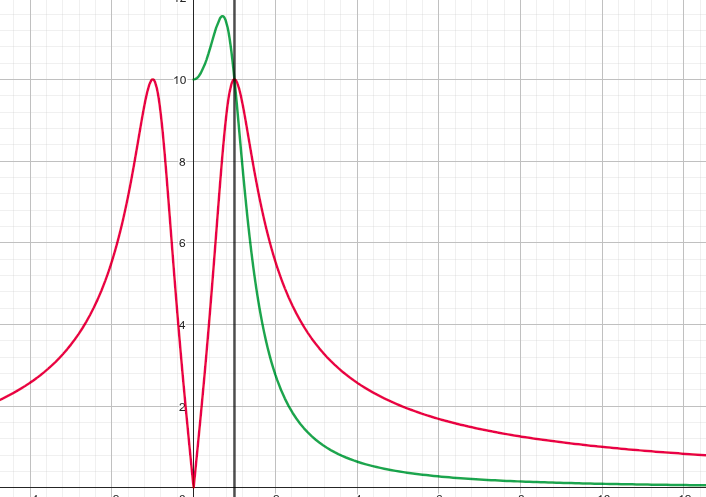
\includegraphics[width=6cm]{img/amplitud forzada.png}
    \caption{forma de la amplitud y velocidad en función de \(\nu\)}
    \label{fig: amplitud forzada}
\end{figure}

En la figura \ref{fig: amplitud forzada} la función verde muestra la amplitud, la roja la velocidad máxima y la recta negra marca el punto donde  \(\nu = \omega_0\). Disponible para modificar en \url{https://www.geogebra.org/classic/xfu3p8ew}

\subsection{Potencia suministrada por la fuerza externa }

En el Oscilador forzado podemos notar de su solución que finalmente alcanza un estado de equilibrio en el que oscila de forma estable, esto puede interpretarse como que la energía del sistema se mantiene constante y como ya sabemos que el amortiguamiento produce disipación de energía, no queda otra explicación más que la fuerza externa debe suministrar la energía disipada por ciclo. \\
\begin{align*}
    \frac{dE}{dt} = 0\\
        \dot{x}(mx + k\ddot{x}) = 0\\
        F\dot{x} = b \dot{x}^{2}
\end{align*}


La potencia instantánea suministrada por la fuerza externa corresponde al producto entre la fuerza externa y la velocidad instantánea.

\begin{align*}
    P = \frac{dW}{dt} = \frac{dW}{dx}\frac{dx }{dt} = Fv
\end{align*}
\begin{align*}
    P &= F_0 \cos \omega t  \frac{F_0}{\|Z_m\|}\cos(\omega t - \theta )\\
    &= \frac{F_0^{2}}{\|Z_m\|}\cos^{2}\omega t \cos\theta + \cos \omega t \sen\omega t \sen\theta
\end{align*}
Luego, puede ser también de interés el estudiar la potencia promedio suministrada, la cual se define como sigue
\begin{align}
    \langle P\rangle = \frac{1}{T} \int_0^{T} P dt 
\end{align}
\begin{align*}
   \langle P\rangle = \frac{1}{T} \int_{0}^{T} \frac{F_0^{2}}{\|Z_m\|}  \cos^{2}\omega t \cos\theta + \cos \omega t \sen\omega t \sen\theta \ dt
\end{align*}
Ahora bien,
\begin{align*}
    \int_{0}^{T} \cos^{2} \omega t dt = \frac{T}{2} 
\end{align*}

y 
\begin{align*}
    \int_{0}^{T} \cos \omega t \sen \omega t \ dt  = 0
\end{align*}
Entonces 
\begin{align*}
    \langle P \rangle = \frac{ F_0^{2}}{2\|Z_m\|}\cos\theta
\end{align*}

Recordemos que \(\theta \) corresponde al argumento de la impedancia, sea \(\theta = \tan^{-1} \frac{m\omega - k/\omega}{b}\)

por lo que la potencia promedio es mayor a medida que la impedancia sea un número complejo mayormente real. Por esto mismo, el el término \(\cos \theta\) en esta expresión puede ser llamado factor de potencia.

\section{Osciladores acoplados}

\subsection{Péndulos unidos por un resorte}
\begin{figure}[h]
    \centering
    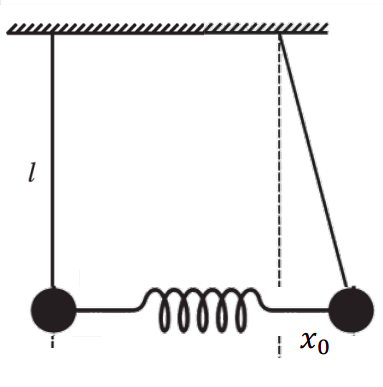
\includegraphics[width=6cm]{img/2 pendulos con resorte.png}
    \caption{2 Péndulos cuyas masa están unidas por un resorte}
\end{figure}
En este caso debemos nuevamente usar la aproximación \(\sen\theta \approx \theta\), además de considerar que la fuerza del resorte va siempre en la dirección angular(perpendicular a la cuerda/varilla) y se estira a lo largo de la circunferencia definida por cada péndulo, usando la segunda ley de Newton para rotaciones
\begin{align*}
    I\ddot{\theta} = \tau
\end{align*}
Obtenemos las siguientes ecuaciones de movimiento para la masa 1 y 2
\begin{align*}
    m_1L^{2} \ddot{\theta}_1 = - m_1gL\theta_1 + kL^{2}(\theta_2 - \theta_1)\\
    m_2L^{2} \ddot{\theta}_2 = - m_2gL\theta_2 + kL^{2}(\theta_1 - \theta_2)
\end{align*}

\begin{figure}[h]
    \centering
    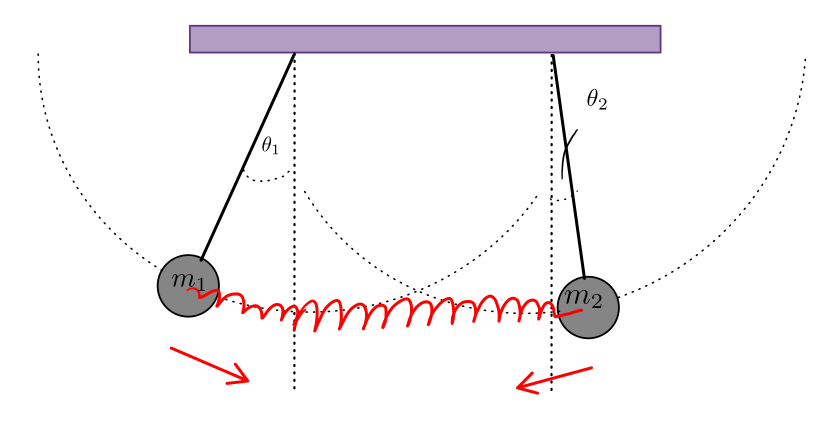
\includegraphics[width=7cm]{img/Pendulo doble con resorte.png}
    \caption{péndulos con sus posiciones y fuerzas}
\end{figure}


Reescribiendo
\begin{align*}
    m_1 \ddot{\theta}_1 = - m_1\frac{g}{L}\theta_1 + k(\theta_2 - \theta_1)\\
    m_2 \ddot{\theta}_2 = - m_2\frac{g}{L}\theta_2 + k(\theta_1 - \theta_2)
\end{align*}
Por simplicidad convengamos que \(m_1 = m_2 = m\) y además definimos las cantidades
\begin{align*}
    \omega_0^{2} = \frac{g}{L} \\\tag{frecuencia natural}
\end{align*}
\begin{align*}
    \omega_c^{2} = \frac{k}{m}\\ \tag{frecuencia del acople}
\end{align*}
\begin{align}
     \ddot{\theta}_1 + \omega_0^{2}\theta_1 + \omega_c^{2}(\theta_1 - \theta_2)  = 0  \label{eq: sistema 2 péndulos a}\\
     \ddot{\theta}_2 +  \omega_0^{2}\theta_2 + \omega_c^{2}(\theta_2 - \theta_1)= 0 \label{eq: sistema 2 péndulos b}
\end{align}
Este es un sistema de ecuaciones diferenciales acopladas, el cual puede resolverse de forma general mediante métodos matriciales, esto se verá más adelante. En este caso se abordará mediante el estudio de sus \textbf{modos normales}. Esto requiere el realizar un cambio de coordenadas que nos permita resolver el sistema más fácilmente.\\

Sumando \eqref{eq: sistema 2 péndulos a} con \eqref{eq: sistema 2 péndulos b} se tiene

\begin{align*}
    \frac{d^{2}}{dt^{2}}(\theta_1 + \theta_2) + \omega_0^{2}(\theta_1 + \theta_2) = 0
\end{align*}
y de restar \eqref{eq: sistema 2 péndulos b} a \eqref{eq: sistema 2 péndulos a} se tiene
\begin{align*}
    \frac{d^{2}}{dt^{2}}(\theta_1-\theta_2) + \omega_0^{2}(\theta_1-\theta_2) + 2\omega_c^{2}(\theta_1-\theta_2) = 0
\end{align*}

Con esto definimos las coordenadas
\begin{align*}
    q_1 = \theta_1 + \theta_2\\
    q_2 = \theta_1 - \theta_2
\end{align*}
Para obtener las ecuaciones desacopladas
\begin{align*}
    \frac{d^{2}q_1}{dt^{2}}  + \omega_0^{2}q_1 = 0\\
    \frac{d^{2}q_2}{dt^{2}}  +(\omega_0^{2} + 2\omega_c^{2} )q_2 = 0
\end{align*}
Las cuales son resolubles con los métodos previamente estudiados.
\begin{align*}
    q_1 &= A \sen(\omega_0 t + \phi_1)\\
    q_2 &= B \sen \left(\omega't + \phi_2\right), \qquad \omega' = \sqrt{\omega_0^{2} + 2\omega_c^{2}}
\end{align*}
Estos modos de nos permiten directamente obtener las ecuaciones de movimiento para cada  masa puesto que se puede revertir el cambio de coordenadas
\begin{align*}
    \theta_1&= \frac{q_1+q_2}{2} \\
    \theta_2 &= \frac{q_1+q_2}{2}
\end{align*}
Además de tener cada uno su propia interpretación física.

\begin{figure}[h]
    \centering
    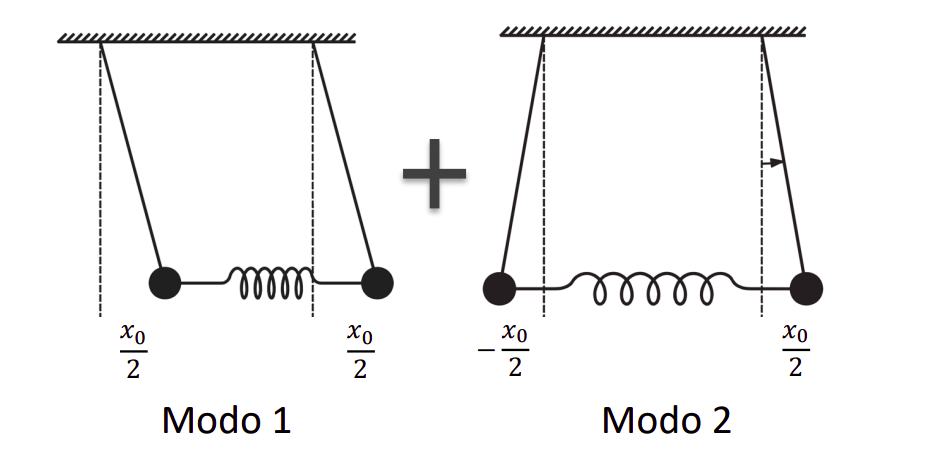
\includegraphics[width=7cm]{img/modos normales péndulo.png}
    \caption{Modos normales}
\end{figure}
 Primero analicemos el modo normal \(q_1\), si el movimiento fuera puramente de esta forma, es decir \(q_2= \theta_1 + \theta_2 = 0 \rightarrow \theta_1 = \theta_2\).\\

 Esto implica que ambos péndulos mantienen siempre la misma inclinación, distancia y por lo tanto, el resorte que los une se mantiene relajado, por lo tanto tiene sentido que la frecuencia de oscilación sea la misma que la de un péndulo simple.\\


El caso de \(q_2 \) con \(q_1= \theta_1 + \theta_2 = 0 \rightarrow q_1 = - q_2\) implica que cuando un péndulo se abre hacia la izquierda, el otro se mueve la misma cantidad pero hacia la derecha lo que produce un movimiento simétrico respecto al punto medio entre ambos. Acá si podemos notar un aumento en la frecuencia, lo que se corresponde con las compresiones y extensiones del resorte uniendo las masas.\\

Cualquier otro tipo de movimiento puede ser expresando como una combinación de estos 2 modos normales.\\

Las soluciones para \(\theta_1\) y \(\theta_2\) corresponden a la interferencia de estas dos soluciones de los modos normales, y como corresponden a oscilaciones de distintas frecuencias presentan el fenómeno de beating estudiada en \ref{subsec: superpocición de oscilaciones colineales}

\subsection{Energía en el sistema acoplado}

Para analizar la energía en el sistema acoplado debemos considerar como siempre tanto la energía cinética como la potencial.
\begin{align*}
    E = K + U
\end{align*}
y debemos ser cuidadosos en considerar todas las partes involucradas sin contar doble.\\

Por ejemplo, para los dos péndulos unidos con un resorte debemos considerar la energía cinética de ambas masas, la energía potencial gravitacional de cada una y además la energía potencial elástica del resorte que las une.
\begin{align*}
    E= \frac{1}{2}mL(\theta_1^{2} + \theta_2^{2}) + mgL(\cos\theta_1 + \cos \theta_2) + kL^{2}(\theta_1 - \theta_2)^{2}
\end{align*}
{\color{red} REVISAR!!!(ojalá agregar ejemplos)}

\subsection{Método matricial  }

Retomando las ecuaciones de los péndulos acoplados
\begin{align*}
    m_1 \ddot{\theta}_1 = - m_1\frac{g}{L}\theta_1 + k(\theta_2 - \theta_1)\\
    m_2 \ddot{\theta}_2 = - m_2\frac{g}{L}\theta_2 + k(\theta_1 - \theta_2)
\end{align*}
o
\begin{align*}
     \ddot{\theta}_1 + \omega_0^{2}\theta_1 + \omega_c^{2}(\theta_1 - \theta_2)  = 0  \\
     \ddot{\theta}_2 +  \omega_0^{2}\theta_2 + \omega_c^{2}(\theta_2 - \theta_1)= 0
\end{align*}

Podemos proponer las soluciones
\begin{align*}
    \theta_1 = \text{Re}(\tilde{A} e^{i\omega t})\\
    \theta_2 = \text{Re}(\tilde{B} e^{i\omega t})
\end{align*}




\begin{thebibliography}{99}
    \bibitem{Clases} Clases del profesor Renato Saavedra
    \bibitem{MIT Howard Georgi} The Physics of Waves, Howard Georgi. \href{https://ocw.mit.edu/courses/8-03sc-physics-iii-vibrations-and-waves-fall-2016/ef731c1b91d77a6db003f6c27e300d25_MIT8_03SCF16_Textbook.pdf}{Disponible aquí}
    \bibitem{Pain} THE PHYSICS OF VIBRATIONS AND WAVES, H.J. Pain \href{http://103.76.208.7:8080/jspui/bitstream/123456789/616/1/Pain%20PHYSICS%20OF%20VIBRATIONS%20AND%20WAVES%206-th%20Edition.pdf}{Disponible aquí}
\end{thebibliography}





\end{document}